\documentclass{beamer}
\usepackage{listings}
\lstset{
%language=C,
frame=single, 
breaklines=true,
columns=fullflexible
}
\usetheme[progressbar=frametitle]{metropolis}
\usepackage{appendixnumberbeamer}

\usepackage{booktabs}
\usepackage[scale=2]{ccicons}
\newenvironment{subcolumns}[1]
 {\valign\bgroup\hsize=#1##\cr}
 {\crcr\egroup}
\newcommand{\nextsubcolumn} {\cr\noalign{\hfill}}
\newcommand{\nextsubfigure}{\vfill}
\usepackage{pgfplots}
% \usepgfplotslibrary{dahttps://www.overleaf.com/project/643bb85840671ea17545bc17teplot}

\usepackage{xspace}
\newcommand{\themename}{\textbf{\textsc{metropolis}}\xspace}
\usepackage{subcaption}
\usepackage{url}

\usepackage{tikz}
\usetikzlibrary{arrows.meta,positioning}
\usepackage{pgfplots}
\pgfplotsset{compat=1.17}
\usepackage{tkz-fct}
\usepackage{mathrsfs}
\usepackage{txfonts}
\usepackage{tkz-euclide} 
\usetikzlibrary{calc,math}
\usepackage{float}
\newcommand\norm[1]{\left\lVert#1\right\rVert}
\renewcommand{\vec}[1]{\mathbf{#1}}
\providecommand{\pr}[1]{\ensuremath{\Pr\left(#1\right)}}
\usepackage[export]{adjustbox}
\usepackage[utf8]{inputenc}
\usepackage{amsmath}
\usepackage{mathtools}
\usepackage{xfrac}
\newcommand{\SubItem}[1]{
    {\setlength\itemindent{15pt} \item[-] #1}
}
\title{Real Data Analysis}
\subtitle{MA4740 - Introduction to Bayesian Statistics}
\date{\today}

\author{GROUP - 8}
%\institute{Indian Institute of Technology Hyderabad}
\titlegraphic{\hfill
\includegraphics[height=1.5cm]{Images/iith logo.png}}

\begin{document}
\metroset{block=fill}
\begin{frame}
\titlepage
\end{frame}
\begin{frame}{Team Members}
\begin{itemize}
    \item Kethari Narasimha Vardhan - MA20BTECH11006
    \item Mulugu Vishwanath Sharma - MA20BTECH11010
    \item Prajwaldeep Kamble - MA20BTECH11013
\end{itemize}
\end{frame}
\begin{frame}
\section{Introduction}
\end{frame}
\begin{frame}{Introduction}
   \begin{block}{Abstract}
     This presentation is based on a group project part of the MA4740 - Introduction to Bayesian Statistics course material. The primary goal of this project is to acquire a real-world data set (not synthetic) and execute Poisson Gamma Bayesian Analysis.
   \end{block} 
\end{frame}
\begin{frame}{Introduction}
   \begin{block}{Objective}
    The project includes:
    \begin{itemize}
    \item Real Data Analysis on Dataset:- \\
    - Rainfall in India from 1901 to 2015.
    \item Performing Poisson Gamma Bayesian Analysis on the collected Dataset.
\end{itemize}
   \end{block} 
\end{frame}
\begin{frame}
\section{Data Collection}
\end{frame}
\begin{frame}{Data Collection}
   \textbf{The Dataset}
     \begin{itemize}
    \item The Dataset, Rainfall in India from 1901 to 2015 is based on the Aggregate Rainfall of each state in India from 1901 to 2015. This dataset is collected from Kaggle.
    \item The data includes all the states, the rainfall in every state in every month throughout the years 1901 up till 2015.
    \item Amongst which, we are interested in the rainfall statistics of Telangana State.
\end{itemize}
\end{frame}
\begin{frame}{Glimpse of the Dataset}
\begin{figure}[htp]
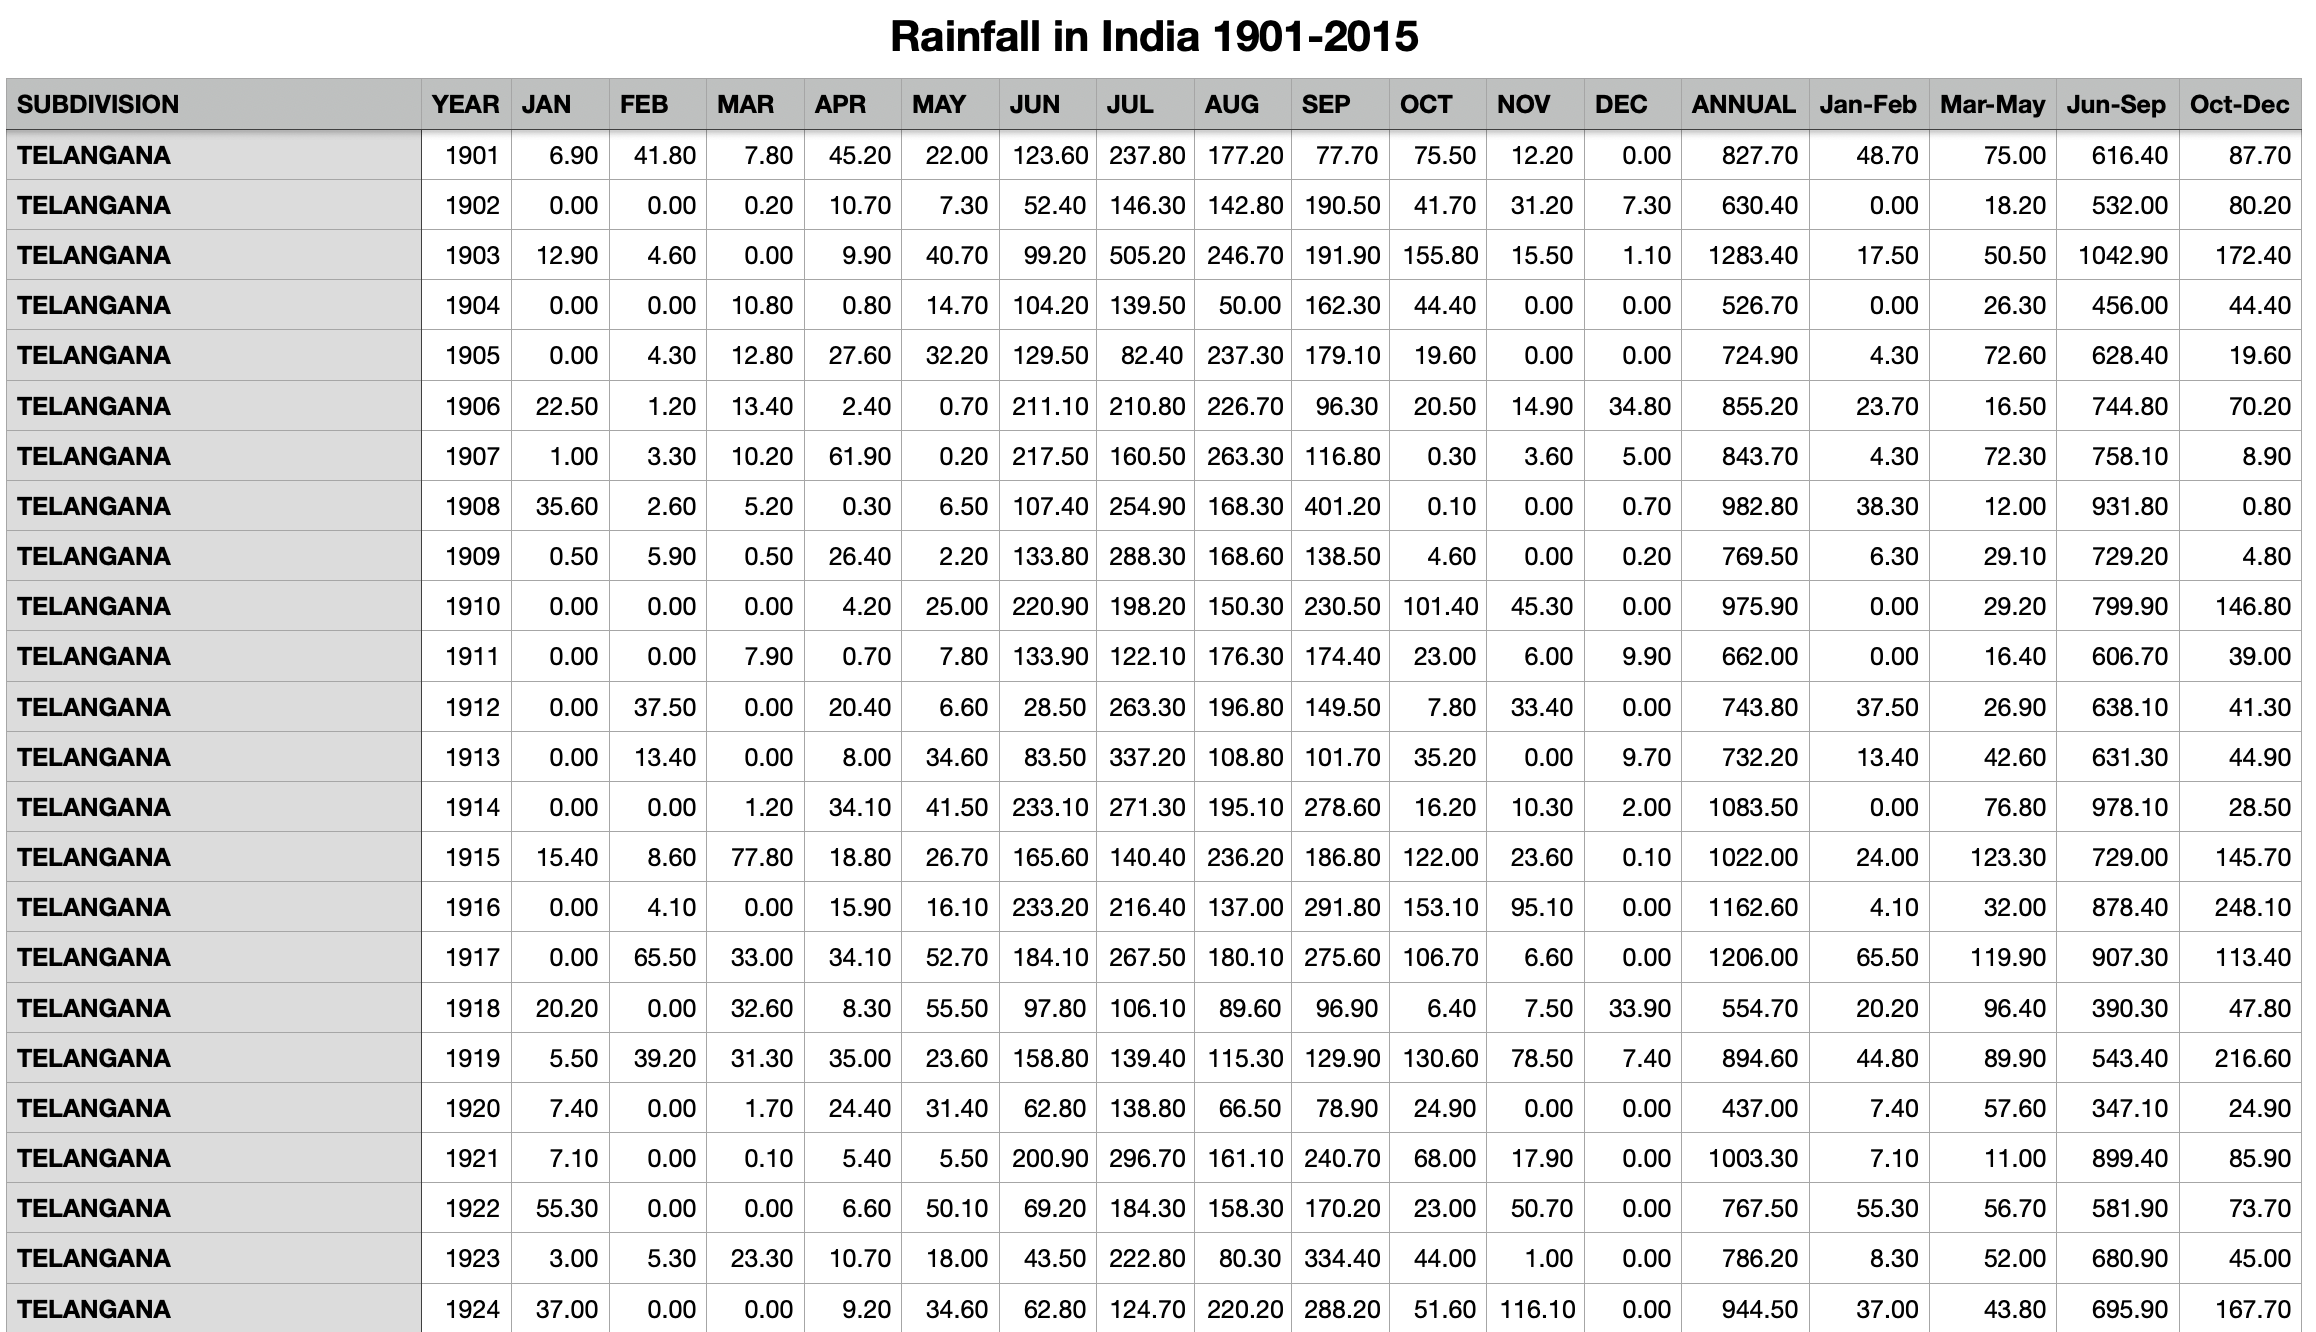
\includegraphics[width=1.05\textwidth]{Images/Glimpse.png}
\caption{Rainfall Statistics in Telangana from 1901 - 1924}
\end{figure}  
\end{frame}

\begin{frame}{Defining variables}
The below representations of the data we used regarding the variables we learned in class.
\begin{align}
    \lambda \sim Gamma(\alpha,\: \beta)\\
    Y \:| \:\lambda \sim Poisson(\lambda)\\
    \lambda \:|\: Y \propto f(Y\:|\:\lambda)* f(\lambda)
\end{align}

Where, \\
\begin{center}
$\lambda = $ Amount of rainfall in a year \\
$Y = $ Data of rainfall over the $n$ years\\
(Random sample of size $n$, $Y_i\:|\:\lambda \sim Poisson(\lambda))$
\end{center}
\end{frame}

\begin{frame}
\section{Poisson Gamma Bayesian Data Analysis}
\end{frame}

\begin{frame}
\section{Prior Distribution}
\end{frame}

\begin{frame}{Prior Distribution}
    \begin{itemize}
        \item The prior data is taken from the dataset from the years 1901 to 1980.
        \item We choose the amount of rainfall in a year ($\lambda$) for the prior data.
        \item We try to fit the prior data to a Gamma Distribution. \\
        We get $\lambda \sim Gamma(\alpha, \:\beta)$.
    \end{itemize}
    \begin{block}{Formula}
        \begin{center}
            $\mu = \cfrac{\alpha}{\beta}$\:, \quad
            $\sigma = \cfrac{\alpha}{\beta^2}$
        \end{center}
        Where, $\alpha$ is the shape hyper-parameter and $\beta$ is the scale hyper-parameter of $Gamma(\alpha, \:\beta).$
    \end{block}
\end{frame}

\begin{frame}{Prior Distribution}
    \begin{itemize}
        \item From the 12 months of data that is collected, the Bayesian Analysis is performed on four months of the year. \\Namely, January, February, March, and April.
        \item After performing the necessary calculations, we get the values of the hyper-parameters $\alpha$ and $\beta$ for these months as
    \end{itemize}
    \begin{block}{Calculations}
        \begin{center}
            $\alpha_{Jan} = 0.37, \quad\beta_{Jan} = 12.07, \quad PriorMean_{Jan} =  4.51$ \\
            $\alpha_{Feb} = 0.62, \quad\beta_{Feb} = 8.39, \quad PriorMean_{Feb} =  5.22$ \\
            $\alpha_{Mar} = 0.41, \quad\beta_{Mar} = 23.29, \quad PriorMean_{Mar} =  9.44$ \\
            $\alpha_{Apr} = 1.1, \quad\beta_{Apr} = 16.44, \quad PriorMean_{Apr} =  18.11$ \\
        \end{center}
    \end{block}
\end{frame}

\begin{frame}{Prior Distribution}
The corresponding Prior Distribution graphs are as follows
\begin{figure}[htp]
\centering
\begin{subcolumns}{0.50\columnwidth}
\begin{subfigure}{0.50\columnwidth}
\centering
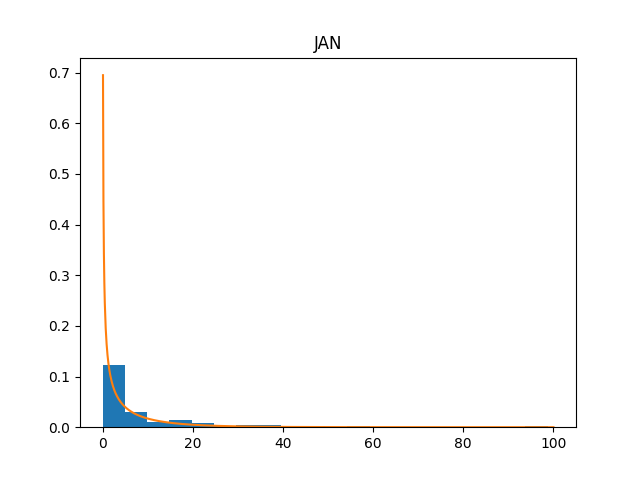
\includegraphics[width=\textwidth]{Images/PriorJAN.png}
\caption{Prior Distribution of January Month}
\end{subfigure}
\nextsubcolumn
\begin{subfigure}{0.5\columnwidth}
\centering
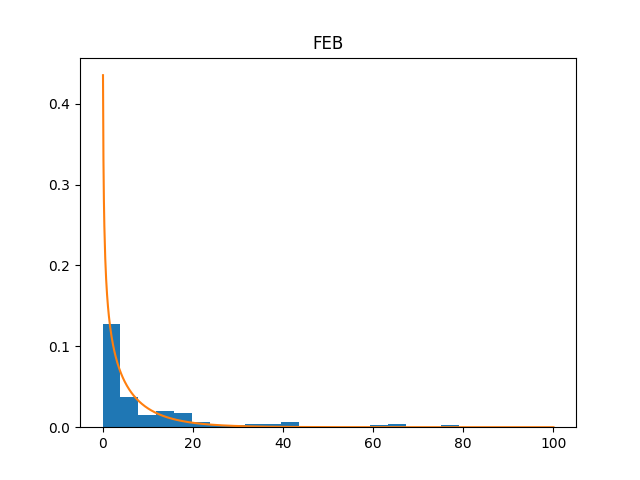
\includegraphics[width=\textwidth]{Images/PriorFEB.png}
\caption{Prior Distribution of February Month}
\end{subfigure}
\end{subcolumns}
\end{figure}
\end{frame}

\begin{frame}{Prior Distribution}
The corresponding Prior Distribution graphs are as follows
\begin{figure}[htp]
\centering
\begin{subcolumns}{0.50\columnwidth}
\begin{subfigure}{0.50\columnwidth}
\centering
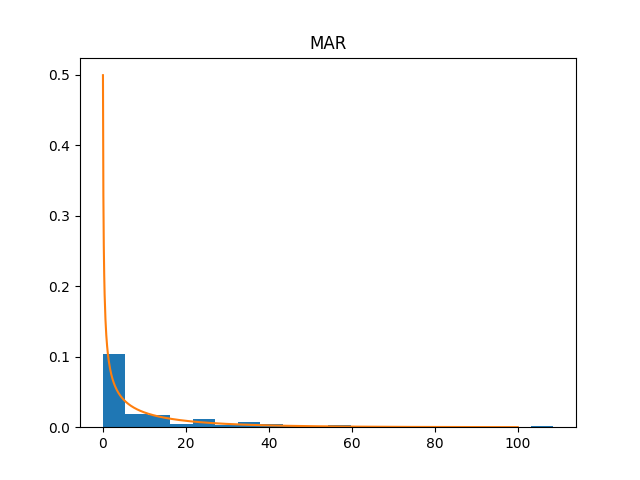
\includegraphics[width=\textwidth]{Images/PriorMAR.png}
\caption{Prior Distribution of March Month}
\end{subfigure}
\nextsubcolumn
\begin{subfigure}{0.5\columnwidth}
\centering
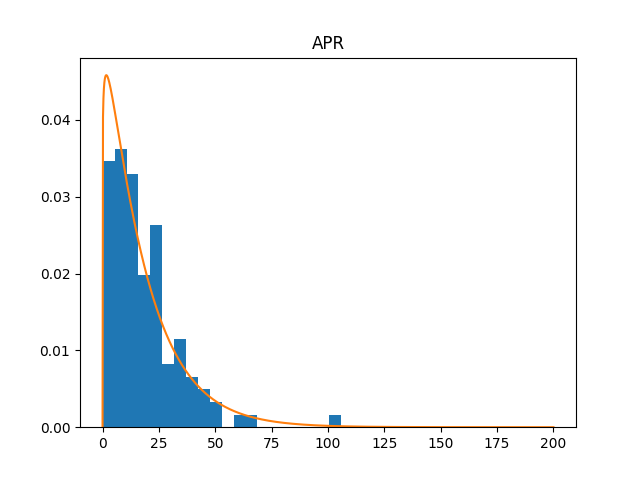
\includegraphics[width=\textwidth]{Images/PriorAPR.png}
\caption{Prior Distribution of April Month}
\end{subfigure}
\end{subcolumns}
\end{figure}
\end{frame}


\begin{frame}
\section{Data-Likelihood Function}
\end{frame}

\begin{frame}{Data-Likelihood Function}
    \begin{itemize}
        \item We require a likelihood function to perform a Poisson Gamma Bayesian Analysis.
        \item We choose $Y\:|\:\lambda \sim Poisson(\lambda)$
        \item Our data consists of the realized values of average rainfall from the years 1981 to 2015.
    \end{itemize}
    \begin{block}{Joint Likelihood}
        \begin{center}
            $P(Y_1=y_1, Y_2=y_2, ..., Y_{35}=y_{35}\:|\:\lambda) = \cfrac{e^{-n\lambda}\lambda^{\Sigma{y_i}}}{\Pi_{i=1}^{i=15}y_i!}$
        \end{center}
    \end{block}
\end{frame}

\begin{frame}{Data-Likelihood Function}
The corresponding Likelihood Function graphs are as follows
\begin{figure}[htp]
\centering
\begin{subcolumns}{0.50\columnwidth}
\begin{subfigure}{0.50\columnwidth}
\centering
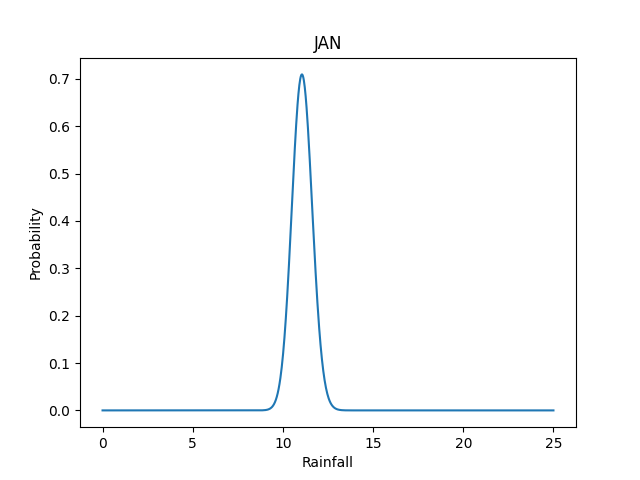
\includegraphics[width=\textwidth]{Images/LikeJAN.png}
\caption{Likelihood for January Month}
\end{subfigure}
\nextsubcolumn
\begin{subfigure}{0.5\columnwidth}
\centering
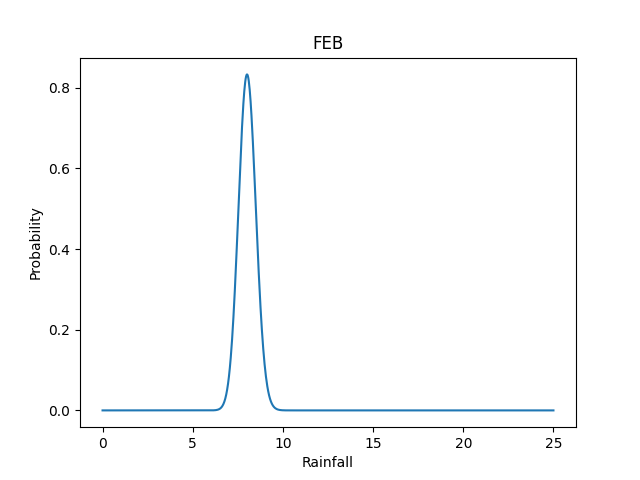
\includegraphics[width=\textwidth]{Images/LikeFEB.png}
\caption{Likelihood for February Month}
\end{subfigure}
\end{subcolumns}
\end{figure}
\end{frame}

\begin{frame}{Data-Likelihood Function}
The corresponding Likelihood Function graphs are as follows
\begin{figure}[htp]
\centering
\begin{subcolumns}{0.50\columnwidth}
\begin{subfigure}{0.50\columnwidth}
\centering
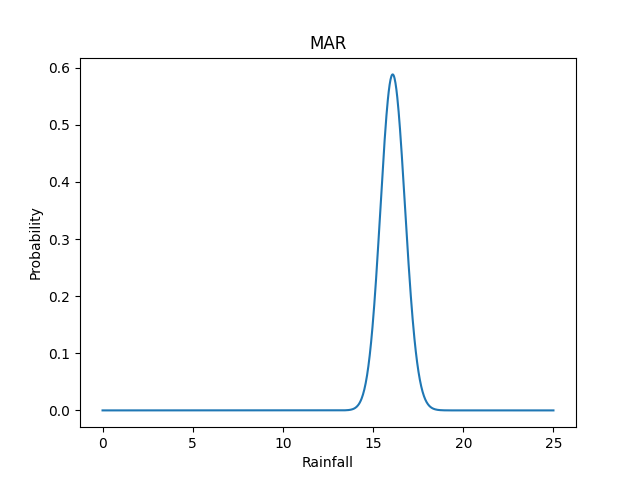
\includegraphics[width=\textwidth]{Images/LikeMAR.png}
\caption{Likelihood for March Month}
\end{subfigure}
\nextsubcolumn
\begin{subfigure}{0.5\columnwidth}
\centering
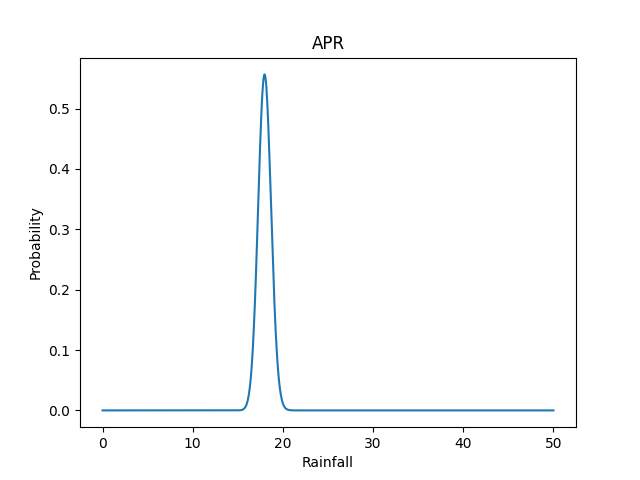
\includegraphics[width=\textwidth]{Images/LikeAPR.png}
\caption{Likelihood for April Month}
\end{subfigure}
\end{subcolumns}
\end{figure}
\end{frame}

\begin{frame}
\section{Posterior Distribution}
\end{frame}

\begin{frame}{Posterior Distribution}
    Using the prior distribution and likelihood function, we try to calculate the posterior distribution. We have,
    \begin{block}{Definition}
        If,
        \begin{center}
            Prior: $\lambda \sim Gamma(\alpha,\: \beta)$ \\
            Likelihood: $Y\:|\:\lambda \sim Poisson(\lambda)$ \\
        \end{center}
        Then, 
        \begin{center}
            Posterior: $\lambda \:|\: Y \sim Gamma(\alpha + \Sigma y_i, \:\beta + n)$
        \end{center}
    \end{block}
\end{frame}

\begin{frame}{Posterior Distribution}
    Thus, after performing the necessary calculations, we get the following values for $Gamma(\alpha',\:\beta')$, with
    \begin{center}
        $\Sigma y_i = y_1 + y_2 + ... + y_n$ \\ and
        $n = 35$
    \end{center}
    \begin{block}{Calculations}
        \begin{center}
            $\alpha'_{Jan} = 387.77, \quad \beta'_{Jan} = 47.07, \quad PosteriorMean = 8.24$ \\ 
            $\alpha'_{Feb} = 281.52, \quad \beta'_{Feb} = 43.39, \quad PosteriorMean = 6.49$ \\ 
            $\alpha'_{Mar} = 563.91, \quad \beta'_{Mar} = 58.29, \quad PosteriorMean = 9.67$ \\ 
            $\alpha'_{Apr} = 630.4, \quad \beta'_{Apr} = 51.44, \quad PosteriorMean = 12.26$ \\ 
        \end{center}
    \end{block}
\end{frame} 

\begin{frame}{Posterior Distribution}
The combined graphs of Prior, Likelihood, and Posterior are as follows
\begin{figure}[htp]
\centering
\begin{subcolumns}{0.50\columnwidth}
\begin{subfigure}{0.50\columnwidth}
\centering
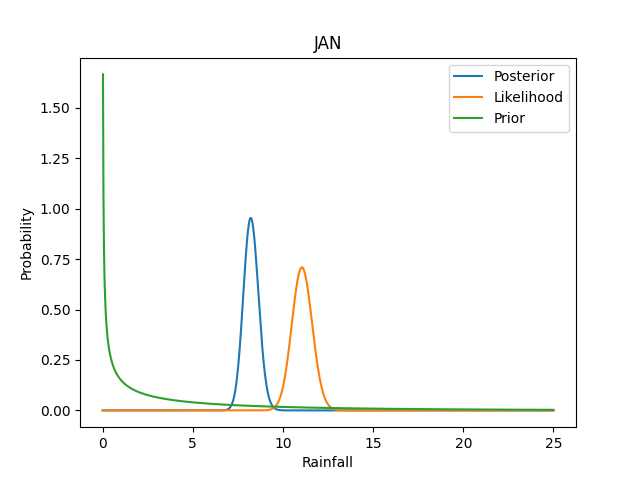
\includegraphics[width=\textwidth]{Images/JAN.png}
\caption{Combined Graph for January Month}
\end{subfigure}
\nextsubcolumn
\begin{subfigure}{0.5\columnwidth}
\centering
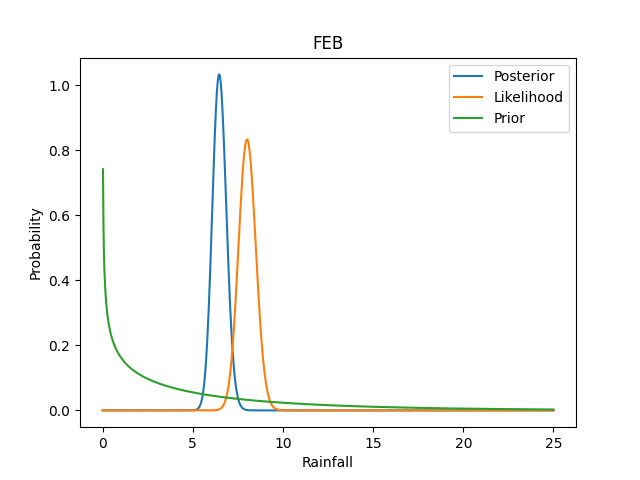
\includegraphics[width=\textwidth]{Images/FEB.png}
\caption{Combined Graph for February Month}
\end{subfigure}
\end{subcolumns}
\end{figure}
\end{frame}

\begin{frame}{Posterior Distribution}
The combined graphs of Prior, Likelihood, and Posterior are as follows
\begin{figure}[htp]
\centering
\begin{subcolumns}{0.50\columnwidth}
\begin{subfigure}{0.50\columnwidth}
\centering
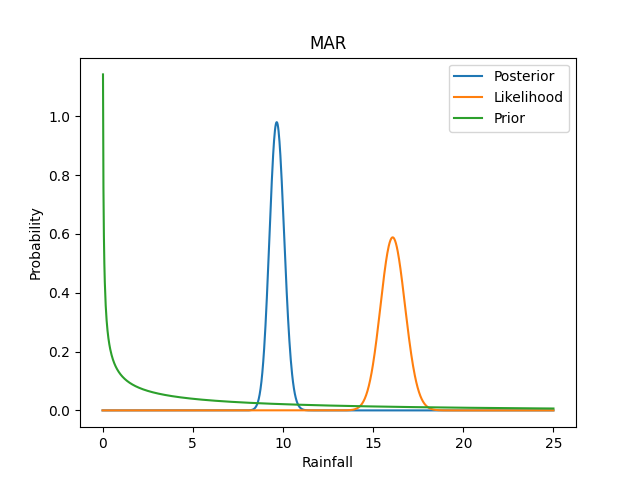
\includegraphics[width=\textwidth]{Images/MAR.png}
\caption{Combined Graph for March Month}
\end{subfigure}
\nextsubcolumn
\begin{subfigure}{0.5\columnwidth}
\centering
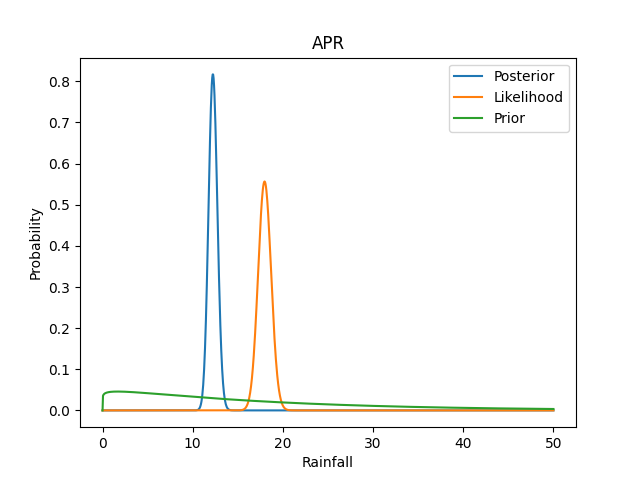
\includegraphics[width=\textwidth]{Images/APR.png}
\caption{Combined Graph for April Month}
\end{subfigure}
\end{subcolumns}
\end{figure}
\end{frame}

\begin{frame}{Conclusion}
If we calculate the means and variances, we can see that the mean of our prior and posterior differ very slightly whereas the variance of prior and posterior differ by a very large margin.

        \begin{center}
            \text{For Jan} \\
            \text{Prior std = } 7.38, \text{Posterior std = } 0.42 \\
            \text{For Feb} \\
            \text{Prior std = } 6.62, \text{Posterior std = }0.39 \\
            \text{For Mar} \\
            \text{Prior std = } 14.83, \text{Posterior std = }0.41 \\
            \text{For Apr} \\
            \text{Prior std = } 17.25, \text{Posterior std = }0.49 \\
        \end{center}
\end{frame}

\begin{frame}{Conclusion}
Below are the $95\%$ confidence intervals for each month.
        \begin{center}
            \text{For Jan} \\
            \text{Prior interval} $\approx \left( 0.0, 25.87 \right)$,\\ \text{Posterior interval} $\approx \left( 7.44, 9.08  \right)$ \\
            \text{For Feb} \\
            \text{Prior interval}$\approx \left( 0.02, 23.75 \right)$,\\ \text{Posterior interval} $\approx \left(5.75, 7.27 \right)$ \\
            \text{For Mar} \\
            \text{Prior interval} $\approx \left( 0.0, 52.19 \right)$,\\ \text{Posterior interval}$\approx \left( 8.89, 10.49 \right)$ \\
            \text{For Apr} \\
            \text{Prior interval}$\approx \left( 0.61, 64.10 \right)$,\\ \text{Posterior interval}$\approx \left( 11.32, 13.23 \right)$ \\
        \end{center}
\end{frame}

\begin{frame}{Inference}
\begin{enumerate}
    \item The confidence interval for the posterior distribution is narrower than the prior's interval and the variance of the posterior distribution is very less than the prior variance so our goal of getting a value more precise than the expectation of the prior is achieved. 
    \item And now if you observe the values of the mean Posterior distributions you can observe that the expected rainfall in Telangana is increasing gradually and if you plot the mean of the posterior distribution of all the months you will encounter a rise in expected rainfall and a drop.
    \item the peak is attained in the rainy season and followed by a  drop which is attained in the winter.
\end{enumerate}

\end{frame}

\begin{frame}
\section{Thank You}  
\end{frame}
\end{document}
